\documentclass[10pt,table]{article}
\usepackage[dvipsnames]{xcolor}
%\usepackage{hyperref}
%\usepackage{amsmath}
\usepackage{tikz}
\usepackage{qtree}
\usepackage{tikz-qtree}
%\usepackage{pgfplots}
\usepackage{listings}
%\definecolor{light-gray}{gray}{0.95}
\usepackage{listings}
\usepackage{setspace}
\renewcommand{\baselinestretch}{1.3} 
\usepackage{graphicx}
\usepackage[export]{adjustbox}
\usepackage{amsmath,amssymb,amsthm,amsfonts,amssymb}
\usepackage{fancyhdr}
\usepackage[b4paper]{geometry}
\usepackage{enumitem}
\usepackage{algorithm}
\usepackage{algpseudocode}
\usepackage{multicol}
\setlength\columnsep{30pt}
\usepackage{setspace}


\setlength{\parindent}{0pt}
\setlength{\parskip}{5pt plus 1pt}
\setlength{\headheight}{13.6pt}
\newcommand\question[1]{\vspace{1.2em}\hrule\textbf{ #1}\vspace{.5em}\hrule}
\renewcommand\part[1]{\vspace{.10in}\textbf{#1)} \enspace}
\pagestyle{fancyplain}
\fancyhf{}
\renewcommand{\headrulewidth}{1.4pt}
\lhead{\textbf{\ANDREWID }}
\cfoot{\textbf{First Draft } - \thepage   }
\rhead{\rule[-1ex]{0pt}{3.5ex} Hossein Naderi }
\newcommand\ANDREWID{Distributed Queue using $\Theta(\log n)$ Shared Memory Accesses} 
\newcommand\HWNUM{1}
\newtheorem{theorem}{Theorem}
\newtheorem{lemma}[theorem]{Lemma}
\theoremstyle{definition}
\newtheorem{definition}{Definition}
\algnewcommand\algorithmicforeach{\textbf{for each}}
\algdef{S}[FOR]{ForEach}[1]{\algorithmicforeach\ #1\ \algorithmicdo}

\begin{document}

\question{Design}
%We store an array of information blocks in each node of the tournament tree that will help us to do Get, Order queries. In merge steps of node n process p reads child left \& right the node n and create a block of info for the new operations in the children. After creating the block the process tries to CAS it to the end of the $n$'s array. Note that ordering is from left to right and from now on when we say $n$ we mean the value on node $n$.


\begin{center}
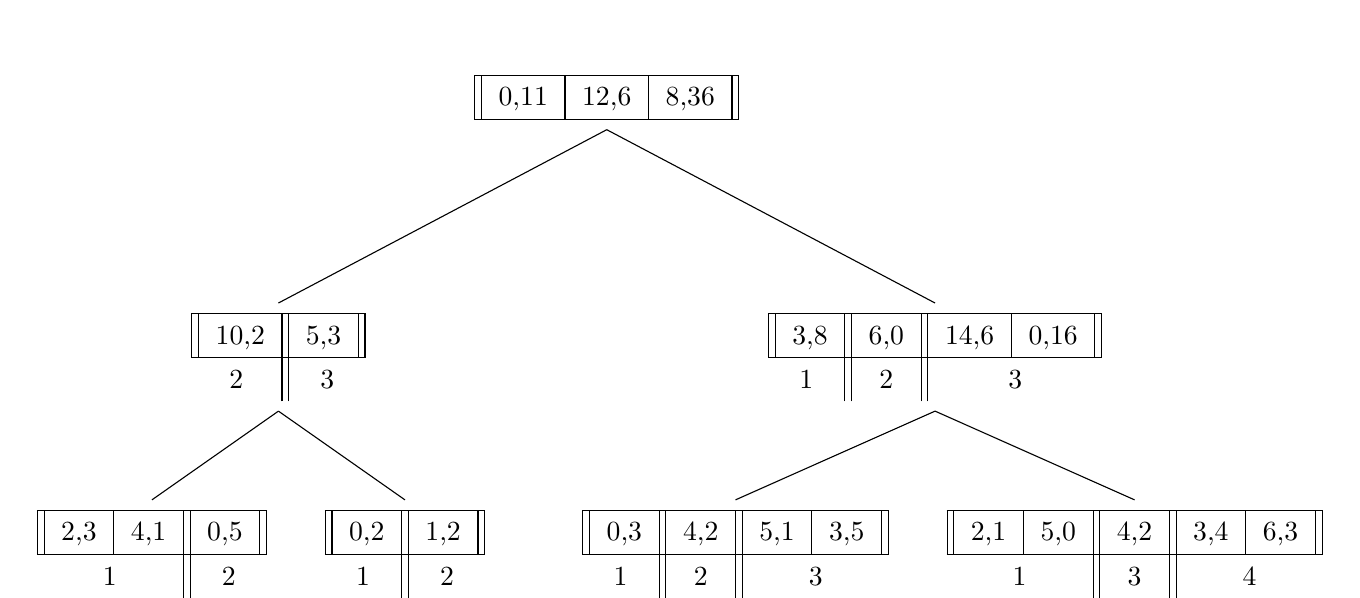
\begin{tikzpicture}[level 1/.style={level distance=3.3cm,sibling distance=1cm},
	level 2/.style={level distance=2.5cm,sibling distance=0.5cm}]
  

\Tree [.{\begin{tabular}{||c|c|c||}  \hline 0,11 & 12,6 & 8,36 \\ \hline\end{tabular}}
 [.{\begin{tabular}{||c||c||}  \hline 10,2 & 5,3 \\  \hline \multicolumn{1}{c||}{2} & \multicolumn{1}{c}{3} \end{tabular}}
 [.{\begin{tabular}{||c|c||c||}\hline 2,3 & 4,1 & 0,5 \\\hline\multicolumn{2}{c||}{1} & \multicolumn{1}{c}{2}\end{tabular}} ]
  [.{\begin{tabular}{||c||c||}  \hline 0,2 & 1,2 \\  \hline \multicolumn{1}{c||}{1} & \multicolumn{1}{c}{2} \end{tabular}} ] ]
          [.{\begin{tabular}{||c||c||c|c||}  \hline 3,8 & 6,0 & 14,6 & 0,16 \\ \hline \multicolumn{1}{c||}{1} & \multicolumn{1}{c||}{2} & \multicolumn{2}{c}{3}\end{tabular}}
           [.{\begin{tabular}{||c||c||c|c||}  \hline 0,3 & 4,2 & 5,1 & 3,5 \\ \hline \multicolumn{1}{c||}{1} & \multicolumn{1}{c||}{2}& \multicolumn{2}{c}{3}\end{tabular}} ]
            [.{\begin{tabular}{||c|c||c||c|c||}  \hline 2,1 & 5,0 & 4,2 & 3,4 & 6,3 \\ \hline \multicolumn{2}{c||}{1} & \multicolumn{1}{c||}{3} & \multicolumn{2}{c}{4}\end{tabular}} ] ] ]

\end{tikzpicture}
\end{center}

%\begin{center}
%\begin{tikzpicture}[level 1/.style={level distance=3cm,sibling distance=2cm}]
%
%\Tree[.{\begin{tabular}{c|c|c|c|c|c}
%  \multicolumn{2}{c|}{enq} & \multicolumn{2}{c|}{deq} & \multicolumn{2}{c}{nill-deq} \\
%  \hline
%5 & 7 & 3 & 4 & 2 & 1 
%\end{tabular}}
%{\begin{tabular}{c|c|c|c|c|c}
%  \multicolumn{2}{c|}{enq} & \multicolumn{2}{c|}{deq} & \multicolumn{2}{c}{nill-deq} \\
%  \hline
%2 & 3 & 0 & 3 & 1 & 0 
%\end{tabular}}
%{\begin{tabular}{c|c|c|c|c|c}
%  \multicolumn{2}{c|}{enq} & \multicolumn{2}{c|}{deq} & \multicolumn{2}{c}{nill-deq} \\
%  \hline
%5 & 2 & 1 & 3 & 2 & 1 
%\end{tabular}} ]
%\end{tikzpicture}
%\end{center}
%





%This is a tournament tree and cells between $||$ are the ones that are propagated together as a block from a child. Tuple(l,r) in a node means l element from left and r elements from right child.



%Each block consists this information for mentioned queries on the tournament tree:
%\begin{itemize}
%  \item $get(i)$: $enq_i,\, deq_i,\, deq\,nill_i$
%  \begin{itemize}
%    \item $\#left \;ops$
%    \item $\#right \;ops$
%    \item $\#left \;enqs$
%    \item $\#right \;enqs$
%    \item $\#left \;deqs$
%    \item $\#right \;deqs$
%    \item $\#left \;deq\,nill_is$
%    \item $\#right \;deq\,nill_is$
%  \end{itemize}
%  \item $index(op)$:
%\end{itemize}

\pagebreak

\begin{algorithm}
\caption{Main Algorithm}\label{alg}
\begin{algorithmic}[1]
\onehalfspacing
%\begin{multicols}{2}


\Statex Shared Objects
%\Statex \hspace{\algorithmicindent}T: Tournament Tree
\Statex \hspace{\algorithmicindent}n: node
\Statex \hspace{\algorithmicindent}\hspace{\algorithmicindent}n.parent: parent of n
\Statex \hspace{\algorithmicindent}\hspace{\algorithmicindent}n.left: left child of n
\Statex \hspace{\algorithmicindent}\hspace{\algorithmicindent}n.right: right child of n
\Statex \hspace{\algorithmicindent}\hspace{\algorithmicindent}n.last: index of the last block in the array
\Statex \hspace{\algorithmicindent}\hspace{\algorithmicindent}n.blocks: array for block objects of n
\Statex \hspace{\algorithmicindent}\hspace{\algorithmicindent}\hspace{\algorithmicindent}block.enq: integer tuple(left, right) 
\Statex \hspace{\algorithmicindent}\hspace{\algorithmicindent}\hspace{\algorithmicindent}block.deq: integer tuple(left, right) 
%\Statex \hspace{\algorithmicindent}\hspace{\algorithmicindent}n.done(type): \# n's propagated operations of the given type
%\State \hspace{\algorithmicindent}\hspace{\algorithmicindent}\hspace{\algorithmicindent}n.done(enq) $\leftarrow$  $\sum_{block \in n.parent.blocks} block.enq.left$ \Comment{if n is the left child}
%\Statex \hspace{\algorithmicindent}\hspace{\algorithmicindent}n.new(type): \# n's not propagated operations of the given type
%\State \hspace{\algorithmicindent}\hspace{\algorithmicindent}\hspace{\algorithmicindent} i$\leftarrow$ \Call{Search}{n, deq, n.done(deq)} 
%\State \hspace{\algorithmicindent}\hspace{\algorithmicindent}\hspace{\algorithmicindent} n.new(deq) $\leftarrow$ $\sum_{j=i+1}^{n.last} n.blocks[j].deq.left + n.blocks[j].deq.right$
%\Statex \Comment{n.new, n.old are computed together at first of each function calling them and the response is not changing}

%\Statex \hspace{\algorithmicindent}\textit{Each array has a $last$ query which return the first null element of the array. Furthermore each cell of these arrays is a tuple(left,right) called block(iff direction==left then !direction==right).}
%\Statex Local Objects
%\Statex \hspace{\algorithmicindent}op-list: Array
\Statex

\Function{Do}{operation op} 
\State l= p's assigned leaf in tree
\State l.append(op)
\State \Call{Propagate}{l.parent}
\State \Return \Call{Compute}{op}
\EndFunction

%\Statex
%
%\Function{Add}{node n, operation op}
%\Statex\Comment{Adds op to leaf n in TT}
%\State op-list.last $\leftarrow$ op
%\State n.last $\leftarrow$ ()
%\EndFunction

\Statex

\Function{Propagate}{node n}
\Comment{propagates $n$ up to the root}
\State block $\leftarrow$ \Call{Read \& Merge}{n}

\If{not \Call{CAS}{n.last, n.last, n.last+1}}
\State \Call{CAS}{n.last, n.last, n.last+1}
\EndIf
\State blocks[last] $\leftarrow$ \Call{Read \& Merge}{n}

\If{n==root} \Return
\Else  \Call{ Propagate}{n.parent}
\EndIf
\EndFunction

\Statex

\Function{Search}{node n, type t, index i , \textit{optional:\{left, right\}}}
\Statex \Comment{returns \#block containing op$_i$ of type $t$ in node $n$}

\EndFunction

\Statex

\Function{Prefix-Sum}{node n, type t, index i , \textit{optional:\{left, right\}}}
\Statex \Comment{returns \#ops before op$_i$ of type $t$ in node $n$}

\EndFunction
\Statex


\end{algorithmic}
\end{algorithm}
\pagebreak
\begin{algorithm}
\caption{Main Algorithm Continued}\label{alg}
\begin{algorithmic}[1]
\onehalfspacing


\Function{Read \& Merge}{node n}

%\If{type==\{ENQ, DEQ\}}\Return tuple(new$_{left}$, new$_{right}$)

\State new-block $\leftarrow$  \{\}

\ForEach{type $\in$ \{enq, deq\}}


%\Statex\Comment{returns block info of $n$'s children new ops of given type}
%\State done$_{left}$ $\leftarrow$  $\sum_{block \in n.blocks} block.enq.left$
%\State done$_{right}$ $\leftarrow$ $\sum_{block \in n.blocks} block.enq.right$
%\Statex \Comment{count how many are already in n}
%
%\State i$_{left}$ $\leftarrow$ \Call{Search}{n.left, type, done$_{left}$}
%\State i$_{right}$ $\leftarrow$ \Call{Search}{n.right, type, done$_{right}$}
%\Statex \Comment{calculate till which block of each child is done yet}
%
%\State new.type$_{left}$ $\leftarrow$ $\sum_{j=i_{left}+1}^{n.left.last} n.left.blocks[j].type$
%\State new.type$_{right}$ $\leftarrow$ $\sum_{j=i_{right}+1}^{n.right.last} n.right.blocks[j].type$
%\Statex \Comment{computes new ops count}

\State new-block.type $\leftarrow$ \big(n.left.new(type), n.right.new(type)\big)
\EndFor 

\State overall-left $\leftarrow$ \big(n.left.done(enq) - n.left.done(deq) + n.left.done(nill-deq)\big) + n.left.new(enq) - n.left.new(deq) + n.left.new(nill-deq)

\State overall-right $\leftarrow$ \big(n.left.done(enq) - n.left.done(deq) + n.left.done(nill-deq)\big) + n.left.new(enq) - n.left.new(deq) + n.left.new(nill-deq)

\State \Return tuple\big($-$overall-left, $-$overall-right\big)

\EndFunction


\Statex

\Function {Get}{node n, index i, type$\in$\{enq, deq\}}
\Comment{returns $op_i$ in the subtree of node $n$}

%\State position $\leftarrow$ min(temp) \textbf{if} i$\leq\sum_{j=0}^{temp} n.\{type\}[j].left + n.\{type\}[j].right$
\State position $\leftarrow$ \Call{Search}{n, type, i}
\State $\#$before-position $\leftarrow$ $\sum_{j=0}^{position-1} n.blocks[j].type.left + n.blocks[j].type.right$
\State direction $\leftarrow$ \big($\#$before-position + n.blocks[position].type.left $\geq i$\big) ? left : right

\Statex \Comment{calculate block position of $i$ and direction of the child}
\If{direction=left}
\State $\#older_{right} \leftarrow$ $\sum_{j=0}^{position-1} n.blocks[j].type.right$
\State \Call{Get}{n.left, $i- \#older_{right}$}
\Else  
\State $\#older_{left} \leftarrow$ $\sum_{j=0}^{position} n.blocks[j].type.left$
\State \Call{Get}{n.right, $i- \#older_{left}$}\EndIf
\EndFunction

\Statex

\Function {Order}{node n, index i, given-type $\in$ \{enq, deq, nill-deq\}}
\Statex\Comment{let $b$ be the $i$th block in $n$,}
\Statex\Comment{returns how many operations of the given type are before $b$'s last operation in the whole ordring}

\If{n==root} \Return \Call{Prefix-Sum}{n, given-type, i}
\ElsIf{type $\in$ \{enq, deq\}}
\State direction $\leftarrow$ (n.parent.left==n) ? left : right 
\State \#self-ops $\leftarrow$ \Call{Prefix-Sum}{n, given-type, i}
\State parent-position $\leftarrow$ \Call{Search}{n.parent, given-type, i, direction} 
\State \Call{Order}{n.parent, parent-position, given-type}
\Else
\Comment{TODO: nill-deq case}
\EndIf
\EndFunction

%\Statex
%
%\Function {Accumulate}{i, type=\{ENQ, DEQ, Nill-DEQ\}}
%\Comment{counts ops with given type before op i}
%\State read root blocks before i and acuumulate the given types before
%\State direction=decide which child to go
%\Call{Accumulate}{i- other child accumulated, direction}
%\EndFunction

\Statex

\end{algorithmic}
\end{algorithm}
\pagebreak
\begin{algorithm}
\caption{Main Algorithm Continued}\label{alg}
\begin{algorithmic}[1]
\onehalfspacing


\Function{Compute}{operation op}\Comment{returns result of operation op}
\State l= op's assigned leaf in tree
\State offset= op's block index in the l
\Comment{TODO:handle other cases(not complete block)}

%\State i $\leftarrow$ \Call{Accumulate}{l, offset, \{ENQ, DEQ\}}
\If{op.type==ENQ} \Return
\Else
\State enqs $\leftarrow$ \Call{Order}{l, offset, \{ENQ\}}
\State deqs $\leftarrow$ \Call{Order}{l, offset, \{DEQ\}}
\State nill-deqs $\leftarrow$ \Call{Order}{l, offset, \{Nill-DEQ\}}
\State \Return{(enqs-deqs+nill-deqs) $>$ 0 ? \Call{Get}{root, enqs-deqs+nill-deqs} : null }
\EndIf
\EndFunction

\end{algorithmic}
\end{algorithm}
%\end{multicols}

\end{document}




